\documentclass[a4paper, 12pt]{article}
\usepackage[utf8]{inputenc}
\usepackage[russian,english]{babel}
\usepackage[T2A]{fontenc}
\usepackage[left=10mm, top=20mm, right=10mm, bottom=15mm, footskip=13mm]{geometry}
\usepackage{indentfirst}
\usepackage{amsmath,amssymb}
\usepackage{graphicx}
\usepackage[italicdiff]{physics}
\usepackage{float}
\usepackage{array}
\usepackage{physics}
\graphicspath{ {shema/} {graphic/} }
\usepackage{caption}
\captionsetup[figure]{name=Рисунок}
  
\title{Отчет по лабораторной работе 1.1.7

Экспериментальное исследование  
равноускоренного движения}

\author{Максим Осипов, Б03-504}
\date{24.09.2025}

\begin{document}
\maketitle

\section{Аннотация}
В данной лабораторной работе проверяется применимость законов равноускоренного движения для тела, скользящего по наклонной плоскости. Эксперимент повторяет классический опыт Галилея. Движение магнита внутри наклонной трубы регистрируется с помощью системы катушек, которые фиксируют моменты его прохождения. Полученная зависимость координаты от времени обрабатывается для определения ускорения. Исследуя, как ускорение зависит от угла наклона плоскости, определяют ускорение свободного падения и коэффициент трения скольжения, а также оценивают погрешности измерений.

\section{Теоретические сведения}
Данная лабораторная работа основана на проверке фундаментальных законов классической механики, сформулированных И. Ньютоном, применительно к движению тела по наклонной плоскости. Это движение является классическим примером прямолинейного равноускоренного движения.

Основным уравнением, описывающим динамику системы, является второй закон Ньютона. Для тела массой 
\textit{m}, движущегося по плоскости, наклоненной под углом \(\theta\) к горизонту, его удобно записать в проекциях на две взаимно перпендикулярные оси: вдоль плоскости (ось OX) и перпендикулярно к ней (ось OY).

Уравнение вдоль оси OX (направленной вдоль плоскости вниз):
\[ m a = m g \sin \theta - f \]
Смысл: Это уравнение описывает причину ускорения. Равнодействующая сила вдоль плоскости равна разности составляющей силы тяжести \(\ m g \sin \theta\), тянущей тело вниз, и силы трения \(\ f\), направленной против движения.

Уравнение вдоль оси OY (перпендикулярно плоскости):
\[ N = m g \cos \theta \]
Смысл: В этом направлении ускорения нет, поэтому сила реакции опоры\(\ N\) уравновешивает составляющую силы тяжести, прижимающую тело к плоскости.

Для описания силы трения скольжения \(\ f\)используется модель сухого трения, согласно которой эта сила пропорциональна силе нормальной реакции опоры:
\[ f = \mu N \], где 
\(\mu\) — коэффициент трения скольжения.

\begin{figure}[h]
\centering
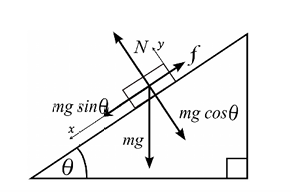
\includegraphics[width=0.4\linewidth]{НАКЛ ПЛОС.png}
\caption{К выводу закона движения по наклонной плоскости }
\label{fig:voltage_current}
\end{figure}





Вывод расчетной формулы для ускорения:
Подставляя выражение для силы трения и силы реакции опоры в первое уравнение, получаем ключевую формулу работы:
\[ a = g (\sin \theta - \mu \cos \theta) \]
Роль в работе: Эта формула является теоретической основой эксперимента. Она предсказывает, что ускорение тела \(\ a\) линейно зависит от тригонометрических функций угла наклона \(\theta\). Константами в этом соотношении являются ускорение свободного падения\(\ g\)  и коэффициент трения \(\mu\), которые нам и предстоит определить.

Прежде чем использовать эту зависимость, необходимо экспериментально подтвердить, что движение является равноускоренным. Кинематика такого движения описывается уравнением:
\[ x(t) = x_0 + v_0 t + \frac{a t^2}{2} \], где\\ \(\ x(t)\) — координата тела в момент времени \(\ t\);\\
\(\ x_0\) — начальная координата;\\
\(\ v_0\) — начальная скорость;\\
\(\ a\) — ускорение (постоянное).

Роль в работе: В эксперименте фиксируются моменты времени \(\ t_n\) прохождения телом известных координат \(\ x_n\). Если, обработав эти данные методом наименьших квадратов, мы получим зависимость \(\ x(t)\), хорошо соответствующую квадратичному закону, это будет доказательством равноускоренного характера движения.\\
Таким образом, теоретическая цепочка эксперимента выглядит так:

Экспериментально (по зависимости \(\ x(t)\)) доказывается, что движение равноускоренное, и для каждого угла \(\theta\) определяется ускорение \(\ a\).

Теоретически ускорение связано с углом наклона формулой \(\ a = g (\sin \theta - \mu \cos \theta)\).

Проведя серию измерений при разных углах \(\theta\) и построив зависимость экспериментальных значений \(\ a\) от \(\theta\), можно, используя метод наименьших квадратов, определить из этой зависимости искомые константы \(\ g\) и \(\mu\), чем и завершается проверка применимости законов механики к данной системе.

\section{Экспериментальная установка }
Лабораторная установка (рис. 2) предназначена для исследования равноускоренного движения тела по наклонной плоскости. Основным элементом установки является пластиковая труба, закреплённая на штативе под переменным углом \(\theta\) к горизонту. Угол наклона регулируется и измеряется с помощью линейки или транспортира.\\

\begin{figure}[h]
\centering
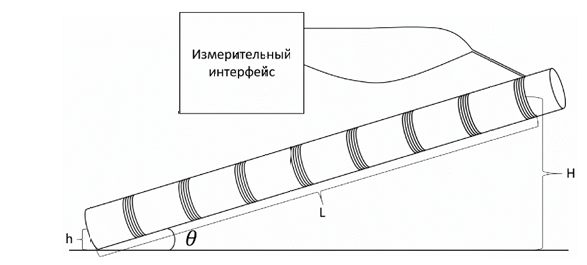
\includegraphics[width=0.8\linewidth]{ЭКСП УСТ.png}
\caption{Экспериментальная установка  }
\label{fig:voltage_current}
\end{figure}






Для вычисления угла используется соотношение:\[
\theta = \arcsin\left(\frac{H - h}{L}\right)
\],где 
\(\ H\) — высота верхнего конца трубы, 
\(\ h\) — высота нижнего конца, 
\(\ L\) — длина трубы.

Вдоль внешней поверхности трубы равномерно размещены десять катушек индуктивности ($n_{\text{max}}$ = 10), соединённых последовательно. Координаты катушек \(\ x_n\)измеряются линейкой относительно начальной отметки (\(\ x_0\)=0). Внутри трубы перемещается неодимовый магнит, играющий роль движущегося тела.

Принцип регистрации движения основан на явлении электромагнитной индукции. При прохождении магнита вблизи катушки возникает импульс напряжения, описываемый законом Фарадея:\[
\mathcal{E} = -\frac{d\Phi}{dt}
\],
где 
\(\varepsilon\) — ЭДС индукции, \(\Phi\) — магнитный поток через катушку. Сигнал имеет характерную форму с двумя экстремумами (максимумом и минимумом), соответствующими приближению и удалению магнита от центра катушки.

Сигналы с катушек усиливаются и преобразуются в цифровую форму с помощью микроконтроллера с АЦП. Компьютерная программа фиксирует моменты времени \(\ t_n\) прохождения магнита через каждую катушку, формируя массив экспериментальных данных 
(\(\ x_n,t_n\)).


Источники погрешностей:

Случайные: неравномерность движения из-за шероховатостей поверхности, боковые колебания магнита, электромагнитные помехи. Уменьшаются многократными измерениями.

Систематические: сопротивление воздуха (вносит погрешность {~1–2\%}), электромагнитное торможение (согласно правилу Ленца). Учитываются при обработке данных.

\section{Цифровая регистрация и обработка результатов}
Регистрация движения магнита осуществляется в цифровой форме. Аналоговый сигнал с катушек усиливается и преобразуется аналого-цифровым преобразователем (АЦП) в массив дискретных значений напряжения \(\ V_i\) в моменты времени \(\ t_i\) с частотой дискретизации ~1 кГц (период ~1 мс).

Обработка данных включает следующие этапы:

1.Определение нулевого уровня сигнала.
На начальном участке данных, где магнит ещё не прошёл ни через одну катушку, вычисляется среднее значение напряжения ⟨\(\ V\)⟩, соответствующее отсутствию сигнала, и его среднеквадратичное отклонение \(\sigma_V\), характеризующее уровень шумов. Величина \(\sigma_V\)  используется для выделения участка сигнала, соответствующего движению магнита.

2.Определение моментов прохождения катушек.
Момент \(\ t_n\) прохождения магнита через 
\(\ n\)-ю катушку соответствует положению локального максимума в оцифрованном сигнале. Начало отсчёта времени \(\ t_0\) и координаты \(\ x_0\) = 0 соответствуют первой катушке. Таким образом, получается массив экспериментальных пар 
(\(\ x_n,t_n\)).

3.Определение параметров движения методом наименьших квадратов.
Для нахождения ускорения \(\ a\) и начальной скорости \(\ v_0\) минимизируется сумма квадратов отклонений:
\[
S = \sum_{n} \left( x_n - v_0 t_n - \frac{a t_n^2}{2} \right)^2 \rightarrow \min
\]
Для аналитического решения методом наименьших квадратов используется замена переменных\\ 
\(\ u = x/t \)
, что приводит к линейной зависимости:
\[
u = v_0 + \frac{a}{2} t
\]

В координатах 
(\(\ u,t\)) угловой коэффициент прямой равен 
\(\ \frac{1}{2}a\).

4.Определение ускорения свободного падения и коэффициента трения.\\
Наконец, по результатам серии экспериментов при разных углах из пар 
значений ({\(\ a\),\(\theta\)}) тем же методом наименьших квадратов для теоретической 
зависимости  определяются параметры ускорение свободного падения \(\ g\) 
и коэффициент трения \(\mu\). Для линеаризации зависимости  можно исполь
зовать, например, замену
\[
a' = \frac{a}{\cos\theta}, \quad \tau = \tan\theta
\]
После замены зависимость становится линейной:
\[
a' = g (\tau - \mu)
\]
То есть ускорение свободного падения — это угловой коэффициента 
наклона наилучшей прямой в координатах (\(\ a'\),\(\tau\)), а коэффициент трения — 
пересечение этой прямой с осью абсцисс. 
















\end{document}